\xchapter{Background}{}
\label{cap:background}

This chapter presents related work and background information necessary to understand this thesis. We first introduce concepts of profiling and instrumentation, then dive into some aspects of the Java Virtual Machine (JVM for short). We follow by presenting a search engine that runs on top of the JVM and concepts related to Linux power governors. Finally, we discuss related work.

\section{Instrumentation}

\emph{Software instrumentation} is a technique that adds auxiliary code to an existing computer program. Instrumentation can be performed either statically (i.e., at compile-time) or dynamically (i.e., at runtime). Static instrumentation is accomplished by modifying the source code or rewriting the application target binary, and dynamic instrumentation is performed after the binary is in-memory \cite{kempf2007instrumentation}.

\emph{Function hooking} is an instrumentation technique by which function calls are intercepted to perform additional operations before or after the function is invoked \cite{lopez2017survey}.

Instrumentation has many applications, such as in profiling, debugging, program analysis, code coverage, and just-in-time compilation \cite{graham1982gprof,zhao2008debug,seward2005memcheck,ivankovic2019googlecov,openjdktier}. For example, a profiler might hook every function of an application to measure and report its execution time.

\section{Profiling}

\emph{Software profiling} is a form of dynamic program analysis used to measure the performance characteristics of a computer program. A profiler can estimate a range of metrics, such as execution time, memory usage, and energy consumption \cite{graham1982gprof,reiss2009visualizing,pathak2012energy}.

Profilers are typically used to identify code blocks where most of the application's time is spent. Once identified, these hot paths can be improved, either manually (i.e., by a programmer) or automatically (i.e., through an algorithm). An optimizing compiler, for example, might use a profile to make more informed decisions or optimize certain functions more aggressively \cite{pettis1990guided}.

CPU profilers can be classified as sampling profilers, in which threads are interrupted once in a while to take samples of its execution, and instrumenting profilers, where the program's code is modified at critical locations to include the reporting of statistics. Sampling profilers typically produce much lower runtime overhead than the instrumented counterpart \cite{moseley2007shadow}.

\subsection{Sampling in Unix-like Systems}

Sampling profilers need to sample the call stack of a thread every few milliseconds. A common way to achieve this on Unix-like systems is to have an application-wide timer that notifies its expiration through a signal. The \code{SIGPROF} signal and \code{ITIMER_PROF} timer are typically used for this purpose. Once the signal is received, the call stack is sampled by walking on the stack of the running thread.

The code executed in the signal handler must be carefully crafted to be \emph{async-signal-safe} \cite{signalsafety}. Async-signal-safe operations are guaranteed not to interfere with operations in the interrupted thread. For example, signals may produce deadlocks if they try to hold the same locks as the interrupted thread. As such, async-signal-safe code is limited to primitive memory operations and a subset of system calls. Given this limitation, profiling signal handlers typically publish the acquired samples to a separate worker thread through an async-signal-safe data structure.


\section{Java Virtual Machine}

The \emph{Java Virtual Machine} is an abstract computing machine. Its primary purpose is to execute code independently of the host hardware and operating system \cite{jvmspec}\nocite{venners1998inside}. This machine has an instruction set and a set of memory areas. There are several implementations of the JVM. Some are in hardware \cite{picojava}, but most are software-based \cite{hotspot, j9, zing}. Oracle's HotSpot is the most popular of these implementations.

\emph{Java} is an object-oriented programming language that compiles to the JVM instruction set. Java found wide popularity in the software industry due to the characteristics of the Java Virtual Machine \cite{kumar2017survey}. Several other programming languages can target the JVM, such as Scala, Clojure, JRuby, and Jython \cite{li2013hosted}.

\subsection{Execution Pipeline}

A program targeting the JVM compiles into a set of class files. A \textit{class file} is a binary format containing JVM instructions (or \emph{bytecode}), symbol tables, and other ancillary information. Class files are loaded, linked, and initialized by the JVM's \emph{class loader}.

The JVM executes classes once they are loaded. Most software implementations employ a just-in-time compiler \cite{kotzmann2008design}\nocite{paleczny2001java}. Bytecode compiles into the host machine instruction set as it gets interpreted. The compiled code can execute with performance characteristics comparable to programming languages natively compiled to machine code \cite{gherardi2012java,taboada2013java}.

Just-in-time compilers may employ profile-guided optimizations. Oracle's HotSpot, for example, performs tiered compilation \cite{java7tier}. It has four levels of compilation which optimizes and deoptimizes functions between levels as the application profile evolves. HotSpot's JIT constructs profiles through instrumentation of method invocations, and loop backedges \cite{openjdktier}.

The Java Virtual Machine features automatic memory management through garbage collection \cite{pufek2019gc}. An unreachable instance of an object is automatically classified as garbage and freed from memory.

\subsection{Java Native Interface}

The \emph{Java Native Interface (JNI)} is an application programming interface (API) that allows JVM bytecode to interoperate with native machine code \cite{jni}. This library can invoke functions written in natively compiled programming languages such as C++ from within a Java program.

Native methods are declared in the Java program, and during class loading, the JVM binds that method to a symbol of a dynamic link library. Listings~\ref{lst:jni_example_java} and \ref{lst:jni_example_cpp} present an example of this interaction.

\begin{figure}[b]
\par\noindent\begin{minipage}[t]{.45\textwidth}
\lstinputlisting[language=Java,frame=tlrb,label=lst:jni_example_java,captionpos=b,caption={Example of a Java program containing the declaration of a native method \code{foo}. The program also loads the dynamic library \code{qux} during class loading.}]{src/listing/JNIExample.java}
\end{minipage}\hfill
\begin{minipage}[t]{.5\textwidth}
\lstinputlisting[language=C++,frame=tlrb,label=lst:jni_example_cpp,captionpos=b,caption={Example of a C++ program exporting a symbol that can be bound to a Java native method. The exported symbol contains the \code{Java} prefix, the package, class, and the method names defined in the Java program. The native method receives the JNI environment, the Java object instance used in the method call, and the \code{bar} parameter defined in the Java declaration. This program can be compiled into a dynamic link library, e.g., \code{libqux.so} and loaded into the Java program.}]{src/listing/JNIExample.cpp}
\end{minipage}
\caption*{} % used to not put in list of figures
\end{figure}

The JVM has a per-thread \emph{JNI Environment} that native functions can use to interact with the JVM. This environment is passed as an argument to every native method invocation. The environment consists of a pointer to a function table and internal data opaque to the native code. The function table contains function pointers that can be used to interface with the JVM. Figure~\ref{fig:jni_function_table} illustrates the approach.

\begin{figure}[h]
\centering
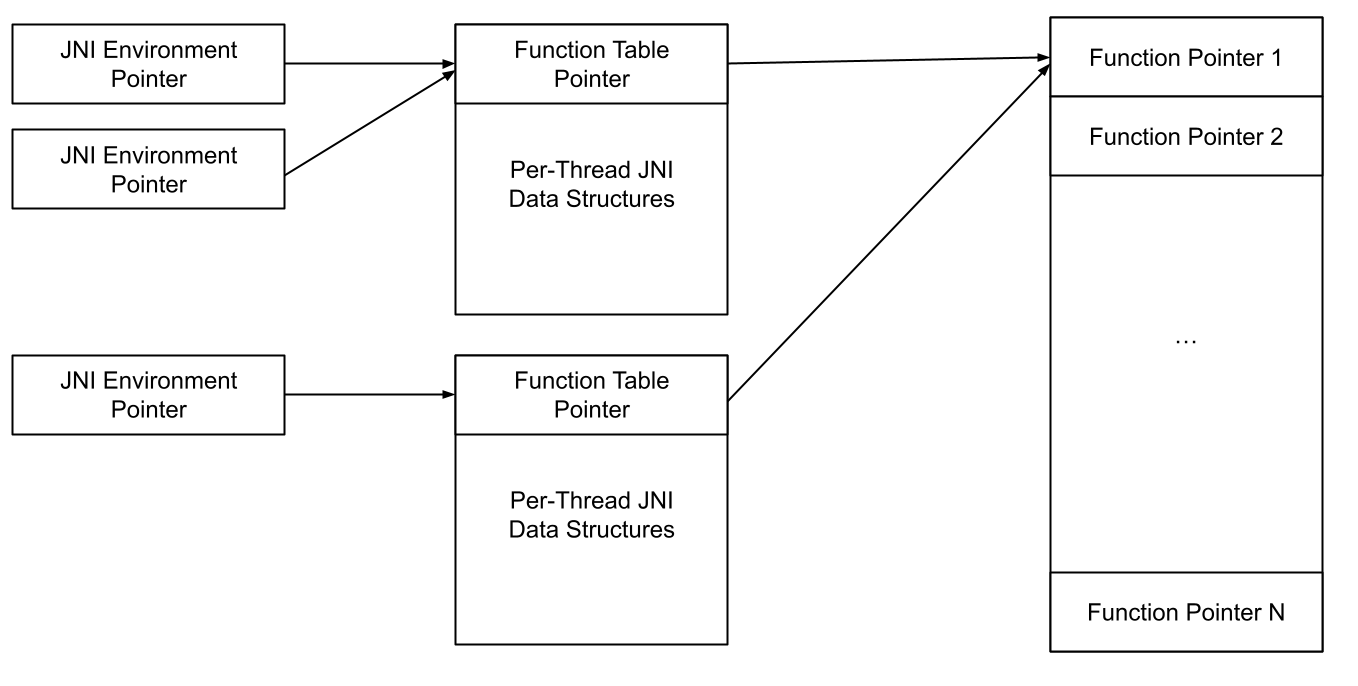
\includegraphics[width=0.81\textwidth]{src/figure/jni_function_table.png}
\caption{The function table approach. Agents have access to an \code{JNIEnv*}, which points to a per-thread JNI environment. This per-thread environment contains a pointer to a function table shared between the environments. The function table holds the JNI interface that clients can use to interact with the JVM.}
\label{fig:jni_function_table}
\end{figure}

The JNI interface provides functionality to invoke Java methods, access object fields, create objects, create references to objects, define classes, throw exceptions, and more. All data type interaction must occur through JNI's data types which map to Java types, e.g., JNI's \code{jobject} maps to Java's \code{Object}.

\subsection{JVM Tool Interface}

The \emph{JVM Tool Interface (JVMTI)} is a programming interface that native agents can use to build development and monitoring tools for the JVM \cite{jvmti}. It provides ways to inspect states and react to events of the VM. Although a JVM implementation is not required to support the JVMTI, most software implementations do.

JVMTI follows most of the approaches in JNI, such as using the same data types and exposing its API through a function table. JVMTI environments can be created by calling JNI's \href{https://docs.oracle.com/en/java/javase/11/docs/specs/jni/invocation.html#getenv}{\code{GetEnv}} function. A native agent is compiled into a dynamic link library and loaded into the VM through command line options. The agent's dynamic library should include the native symbols \code{Agent_OnLoad} and \code{Agent_OnUnload}. The VM invokes these functions during initialization and termination, respectively, to offer the agent an opportunity for setup and tear-down. An example agent is shown in Listing~\ref{lst:example_jvmti}.

\subsubsection*{Capabilities}

JVMTI provides several functions that can be invoked from most contexts, e.g., \apijvmtiref{GetStackTrace} and several events that can be used to react to the VM, e.g., \apijvmtiref{MethodEntry}. These functions and events may come at a cost in execution speed, start-up time, and memory footprint. For this reason, JVMTI does not provide any capability by default. During \code{Agent_OnLoad}, the agent must add (through JVMTI's \apijvmtiref{AddCapabilities}) the capabilities it needs (e.g. \apijvmtiref{can_generate_method_entry_events}).

\subsubsection*{Events}

In addition to capability setting, events of interest can be enabled (and disabled) by calling JVMTI's \apijvmtiref{SetEventNotificationMode}. The event's callback functions can be set with \apijvmtiref{SetEventCallbacks}. Event callbacks receive their JNI and JVMTI environments as arguments, plus additional information related to the event.

\subsubsection*{Environment Disposal}

A JVMTI environment can be disposed of explicitly by calling \apijvmtiref{DisposeEnvironment} or implicitly during agent unloading. During disposal, the environment capabilities are automatically relinquished and its events disabled. Memory and any other additional resources the agent allocates must be freed manually.

\lstinputlisting[language=C++,frame=tb,float,floatplacement=b,caption={Example of a JVMTI agent that intercepts every Java method entry. Agent setup creates a JVMTI environment and requests the necessary capabilities from it. Then, the method entry event is enabled, and its callbacks are set. Error handling is omitted for brevity.},label=lst:example_jvmti]{src/listing/example-jvmti.cpp}.

\subsection{Safepoints}

A \emph{safepoint} is a point of execution in which all root object references are known, and heap object contents are consistent \cite{hotspotglossary}. The most popular JVM implementations use safepoints to assist in implementing operations such as garbage collection, thread dumps, and compiler deoptimization \cite{lin2015yieldpoint}.

A thread is in a safepoint while performing I/O, in between two interpreted bytecode instructions, when running native code, when contended or waiting in a lock, and at specific points of JIT-compiled code \cite{wakart2015safepoints}.

\subsubsection*{Safepoint Polls}

JIT-compiled code can only know the root of object references through compiler-generated structures known as garbage collection maps. These maps contain which machine registers and locations of the stack frame the objects are stored. Generating these maps for every instruction would require large amounts of memory and therefore is infeasible. Moreover, object references may be inconsistent across particular instructions. As an alternative, these maps are created only for specific locations known as \emph{safepoint polls}. Safepoint polls are generated at non-inlined method entry/exits, and non-counted loop backedges \cite{hohenseehotspot}.

Whenever the JVM needs to perform an operation that requires a safepoint (e.g., garbage collection), it must bring all threads to a safepoint. It does so by posting a safepoint request. Each executing thread checks the request at the next safepoint poll and pauses its execution. The time needed to bring a set of threads to a safepoint is known as \emph{time to safepoint}. Once all threads are blocked, the VM performs its operation and resumes the interrupted threads when finished.

\subsubsection*{Safepoint Bias}

JVMTI provides \apijvmtiref{GetStackTrace}, \apijvmtiref{GetThreadListStackTrace} and \apijvmtiref{GetAllStackTraces} functions. These functions can be used to get information on the call stack of threads. These operations require threads to be in a safepoint. Several Java profilers are built around these functions, resulting in profiles with \emph{safepoint bias} \cite{mytkowicz2010evaluating}. These profilers are biased towards the location of the next safepoint poll, resulting in, for example, profiles not showing functions that do not have polls, despite their high CPU usage \cite{wakart2016terrible}. These profilers also introduce additional overhead associated with time to safepoint.

Open-source profilers that mitigate the safepoint bias exists \cite{nisbet2019profiling}. \code{perf-map-agent} \cite{perfmapagent} is capable of profiling kernel, native, and JIT-generated code by producing JIT stack maps for Linux's \code{perf} tool. However, it cannot profile interpreted code. \code{honest-profiler} \cite{honestprofiler} uses the \code{AsyncGetCallTrace} undocumented API to circumvent JVMTI's safepoint strategy. It can trace interpreted code but not kernel and native code. \code{async-profiler} \cite{asyncprofiler} is a hybrid of both approaches and can sample native, kernel, interpreted, and JIT-compiled code.

\section{Elasticsearch}

\emph{Elasticsearch} is an open-source search engine built atop Apache Lucene \cite{bialecki2012lucene}, a Java library that executes indexing and querying/scoring functions. Like Lucene, Elasticsearch is written in Java and is mainly responsible for serving the search results through an HTTP interface while allowing Lucene to scale among clusters.

As a distributed application, multiple nodes or machines comprise an Elastichsearch cluster. This cluster handles all the non-Lucene tasks, such as creating and replicating shards, query distribution, and maintenance. Each node contains one or more shards, where each holds a search index.

\section{Frequency Scaling}

\emph{Dynamic Frequency Scaling (DFS)} is a technique for improving power efficiency on modern multi-core systems. The operating frequency of a particular core increases or decreases according to the application's demand. Given that power consumption is linearly proportional to core frequency, a lower frequency results in less power consumption.

Linux implements DFS in its Ondemand governor \cite{pallipadi2006ondemand}, which attempts to minimize energy consumption by changing the CPU speed according to processor utilization thresholds. The Ondemand governor has been Linux's default since kernel 3.4.

The kernel also provides a userspace governor, in which the user chooses a fixed frequency. 

\section{Related Work}

\nocite{kell2012observable}

\subsection{Machine-Code Instrumentation}

Static instrumentation was pioneered by ATOM \cite{srivastava1994atom}. It applies an instrumentation routine to compiled code, wherein tool developers can insert calls into their analysis functions. Following works, such as EEL \cite{larus1995eel}, and Pebil \cite{laurenzano2010pebil} are conceptually similar but improve on usability, platform support, and functionality.

Pin \cite{luk2005pin}, Valgrind \cite{nethercote2007valgrind}, and DynamoRIO \cite{bruening2004dynamorio} are popular trace-based dynamic instrumentation alternatives. They operate by recompiling code with the extra instrumentation as the program executes. The approach can perform worse than static methods but has better ergonomics, including the significant advantage of manipulating every reachable code path, including dynamically linked and dynamically-generated code.

\subsection{Bytecode Instrumentation}

The mentioned systems were built with native applications in mind and cannot manipulate bytecode. Although native code's dynamic instrumentation can influence the interpreter and JIT-compiled code, it cannot expose the specifics of the virtual machine, such as which Java method or variable is accessed.

BCEL \cite{dahm1999bcel}, ASM \cite{bruneton2002asm}, Javassist \cite{chiba2003javassist} and SOOT \cite{vallee2010soot} are popular static instrumentation libraries for JVM bytecode. These tools and their augmentation routines are written in pure Java and can be used during dynamic instrumentation through events exposed by either JVMTI's agents or Java agents. The former uses native code and executes before the JVM bootstraps itself, while the latter is written in Java and, therefore, cannot instrument core runtime classes.

FERRARI \cite{binder2007ferrari} is an instrumentation framework built as a hybrid of static and dynamic techniques. It statically instruments core classes while using a Java agent for the other ones. DiSL \cite{marek2012disl} achieves full dynamic instrumentation by using a separate JVM process for manipulating bytecode. It uses a JVMTI agent to intercept class loading and forward it to another bootstrapped VM.

JNIF \cite{mastrangelo2014jnif} was created to foster native alternatives. It is a static instrumentation library written in and for use by native code. JVMTIPROF uses JNIF and is, to our knowledge, the first fully native dynamic instrumentation framework for Java.

\subsection{Probe-Based Instrumentation}

JVMTIPROF's instrumentation interface is probe-based, notifying clients of specific events instead of providing the power of arbitrary augmentation. Sofya \cite{kinneer2007sofya}, RoadRunner \cite{flanagan2010roadrunner}, and Btrace \cite{btrace} are examples of existing probe-based instrumentation systems for Java. Byteman \cite{dinn2011byteman} provides an efficient Java-based domain-specific language for probing methods. Linux exposes Byteman's probes in SystemTap's \cite{prasad2005stap} scripting language that compiles into kernel modules.

